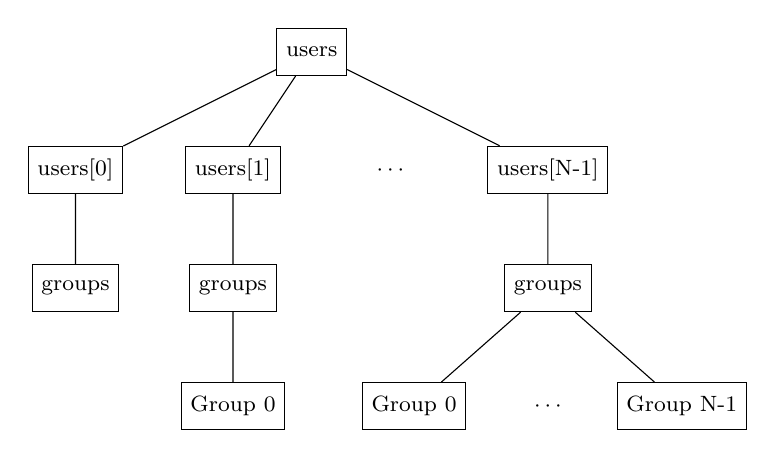
\begin{tikzpicture}
[level/.style={sibling distance=17mm},
 level 1/.style={sibling distance=20mm},
 every node/.style=
   {minimum height=6mm,rectangle,draw=black,font=\footnotesize}]
\node [] {users}
  child {node [] {users[0]}
    child {node [] {groups}
    }
  }
  child {node [] {users[1]} 
    child {node [] {groups}
      child {node [] {Group 0} }
    }
  }
  child {node [draw=none] {$\cdots$} edge from parent[draw=none]}
  child {node [] {users[N-1]}
    child {node [] {groups}
      child {node [] {Group 0} }
      child {node [draw=none] {$\cdots$} edge from parent[draw=none]}
      child {node [] {Group N-1} }
    }
  };
\end{tikzpicture}